%%%%%%%%%%%%%%%%%%%%%%%%%%%%%%%%%%%%%%%%%%%%%%%%%%%%%%%%%%%%%%%%%%%%%%%%%%%%%%%%%

\hypertarget{appendix:a}{} %% uso para este Guia
\renewcommand{\thechapter}{}%
\chapter{APPENDIX A - INTERSECTION ALGORITHMS}
\label{ap:a}
\renewcommand{\thechapter}{A}

\section{Problem}\label{ap:a:problem}

This is only a simple overview to show the importance of the problem and how different algorithms stack against each other.

The problem can be stated as follows: given sets $S_1$ and $S_2$, find the elements that are present in both sets, their intersection, represented as $S_1 \cap S_2$.
Furthermore, each element is ordered as unique, for they represented index positions and are thus always non-zero positive integers.

\section{Algorithms}\label{ap:a:algos}

\textcolor{red}{All wrong for now}

UnorderedSet

Scalar

Li

BinaryLi

std::set\_intersect

SIMD (SS2)


\section{Experiments}\label{ap:a:results}

To search for the best algorithm with real world data, an experiment was performed, much on the same framework as detailed in~\ref{ch:experiment}: C++ code, each test was executed 5 times and the median of the values was taken.
As each technique is efficient with the memory usage, there wasn't much difference to be measured, so only the time necessary to intersect each list was measured.
Each list was generated in interval from $2\times10^6$ to $1\times10^7$, and all algorithms work on randomized ordered lists with the same size.
This spread was intentional to mirror the worst cases in the Frag-Cubing algorithm.

Table~\ref{tab:setresults} showcases a summary of the experiment's results, this time caring only for the necessary time to answer the queries.

\begin{table}[!ht]
  \begin{center}
    \caption{Set Intersection Results, in milliseconds}\label{tab:setresults}
    \begin{tabular}{|c|c|c|c|c|c|c|}
      \hline
      \textbf{Algorithm - N} & \bfseries $2\times10^6$ & \bfseries $4\times10^6$ & \bfseries $6\times10^6$ & \bfseries $8\times10^6$ & \bfseries $1\times10^7$\\
      \hline
      UnorderedSet & 867,802 & 1806,19 & 2586,04 & 3448,11 & 4213,15\\
      \hline
      Scalar & 26,57 & 51,346 & 71,109 & 85,531 & 118,114\\
      \hline
      Li & 26,531 & 45,596 & 66,19 & 86,234 & 108,603\\
      \hline
      BinaryLi & 21,601 & 39,776 & 59,27 & 79,416 & 97,155\\
      \hline
      std::set\_intersect & 17,125 & 34,392 & 51,682 & 67,717 & 84,933\\
      \hline
      SIMD (SS2) & 10,941 & 21,854 & 33,866 & 43,739 & 55,814\\
      \hline
    \end{tabular}
  \end{center}
\end{table}

As the HashSet approach was the slowest approach, \autoref{fig:set_intersection_results} showcases the comparison between the other algorithms, that have comparable performances and are easier to visualize.

\begin{figure}[ht]
  \caption{Set Intersection Algorithm results}\label{fig:set_intersection_results}
  \vspace{6mm}
  \begin{center}
    \resizebox{12cm}{!}{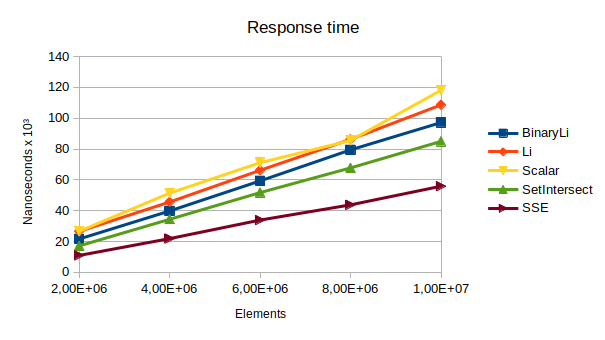
\includegraphics{Figuras/IndexListResult.png}}
  \end{center}
  \vspace{2mm}
  \legenda{Set intersection algorithms response times in milliseconds, ordered by the size of the input relation.}
  \FONTE{Author}
\end{figure}

The SIMD approach is clearly the fastest, however it is also dependant on processor architecture and even though the used SIMD instructions (SS2) are available on almost all modern CPUs, other newer instruction sets might not be, or might have different implementations depending on the CPU vendor, which complicates widespread implementation.

While these tests are interesting, there was not enough time to test some recent benchmarks that found the use of different algorithms and could improve the performance of each, as the use of compressed indexes in \cite{pibiriTechniquesInvertedIndex2019} show.
Furthermore, the SIMD instruction set used here (SSE2) is limited even if it's support is widespread, with other instruction sets (SSE3, AVX, AVX512, etc) being available on modern CPUs and also available for use.

Some recent results that have not been properly explored in the data cube context as of yet: Recursive Universe Partitioning, a technique that uses the possible search space to partition the sets and execute the intersection~\cite{pibiriFastCompactSet2021}; FESIA, which combines the use of previous techniques with different SIMD computation techniques and a bitmap to decide which algorithm is more suitable for use depending on the set size~\cite{zhangFESIAFastSIMDEfficient2020}; and simpler implementations that reduce branch mispredictions~\cite{inoueFasterSetIntersection2014}, and the use of pre-processed dictionaries to greatly aid in the computation~\cite{dingFastSetIntersection2011a}.
There's even an algorithm to compute the set intersection in $\mathcal{O}(1)$ by using a quantum computer~\cite{tianQuantumAlgorithmFinding2019}, however that approach is likely not implementable for any significant dataset in the near future.

Further testing is necessary when dealing with lists of varying sizes, that would showcase the improvements of certain algorithms over others, and the incorporation of these algorithms into a real-world dataset for accurate tests.

